%!TeX root = ../main.tex
\chapter{Quantification of tumor perfusion using DCE-US: impact of mathematical modeling}\label{chapter:PMB}

\section{Abstract}
Dynamic Contrast Enhanced Ultrasound has been proposed to monitor tumor therapy, in complement to volume measurements. To assess the variability of perfusion parameters in  ideal conditions, four consecutive test-retest studies were acquired in a tumor model of mouse, using controlled injections. The impact of mathematical modeling on parameter variability was then investigated. Coefficients of variation (CV) of tissue blood volume (BV) and tissue blood flow (BF) based-parameters were estimated inside 32 sub-regions of the tumors, comparing the log-normal (LN) model with a one-compartment model fed by an arterial input function (AIF) and improved by the introduction of a time delay parameter. Relative perfusion parameters were also estimated by normalization of the LN parameters and normalization of the one-compartment parameters estimated with the AIF, using a reference tissue (RT) region. A direct estimation (rRTd) of relative parameters  based on the one-compartment model without using the AIF was also obtained by using the kinetics inside the RT region.  Results on test-retest studies show that absolute regional parameters have high CV, whatever the approach, with median values of about 30\% for BV, and 40\% for BF. The positive impact of normalization was established, showing a coherent estimation of relative parameters, with reduced CV (about 20\% for BV and 30\% for BF using the rRTd approach). These values were significantly lower ($p<0.05$) when compared to CV of absolute parameters. The rRTd approach provided the smallest CV and should be preferred for estimating relative perfusion parameters. 

\section{Introduction}
Reliable quantification of tumor perfusion is a challenging objective in order to establish cancer diagnosis and to monitor therapy. Tumor perfusion can be assessed through various imaging modalities, including PET, Dynamic Contrast Enhanced (DCE) MR, CT, and ultrasound (DCE-US).

Compared to DCE-MRI, DCE-CT and PET, the main advantages of DCE-US are its real-time, non-ionizing, and cost-effective characteristics. Moreover, as micro-bubbles do not diffuse in the extra-vascular space, DCE-US studies reflect only the tissue vasculature. 
Different acquisition protocols are available including bolus and destruction-replenishment during infusion~\cite{Wei1998tc}. The present work focuses on bolus injections, since this acquisition mode is the most widely used~\cite{Dietrich2012kw}. 

It is currently recommended for bolus DCE-US studies to estimate semi-quantitative parameters using explicit models, such as the Log-Normal model~\cite{Strouthos2010it}. 
However, it was shown that these semi-quantitative parameters were sensitive to various factors~\cite{Tang2011fj}: scanner-related (e.g.~frequency, mechanical index, dynamic range, focal length), patient-related (e.g.~blood pressure, tissue motion, physiological interaction), and bubble-related (e.g.~bubble type, concentration, preparation, injection) factors. The quantification of bolus DCE-US studies thus remains a major challenge.

In an attempt to make quantification of tissue perfusion less sensitive to external factors, quantitative approaches based on indicator dilution theory and commonly used for PET, DCE-MRI or DCE-CT exams~\cite{Tofts1999ih,Wedam2006bi,OConnor2007ku} could be  applied to DCE-US data.
These methods estimate tissue blood volume and  tissue blood flow parameters by performing a specific deconvolution of the tissue time-intensity curve inside the tumor by an Arterial Input Function (AIF) measured in the imaging plane.  Similarly to  what was done in above cited imaging modalities, a compartmental approach was recently proposed for DCE-US ~\cite{Doury2016tk}. Precisely, a one-compartment model was proposed since the contrast agent remains in the blood. This approach defines a set of admissible curves for the transfer function (mono-exponential functions), and the estimation of parameters is then regularized intrinsically. It can thus be distinguished from blind deconvolutions, as recently proposed in DCE-US~\cite{Gauthier2012vc,Jirik2014hv}. Indeed, these  approaches require establishing strong constraints on the transfer functions, due to their large number of unknown parameters.

The present study aimed at comparing different modeling approaches and at studying the reproducibility of perfusion parameters in test-retest measurements on a mouse tumor model, acquired using controlled injections~\cite{Dizeux2016cd}. Three absolute modeling approaches including a Log-Normal model and a one-compartment model without and with a time delay were first compared. In a second time, relative perfusion parameters were defined by normalizing the values obtained in the tumor with values obtained in a reference tissue region, and five relative derived models were studied. 

\section{Materials}

\subsection{Animals}
Murine Lewis Lung Carcinoma (3LL) were used. Tumor fragments (20-40 mm$^3$) were implanted subcutaneously 20 days prior to the experiment in the right flank of four Balb/C mice. All experiments were conducted in accordance with the institutional guidelines and the recommendations for the care and use of laboratory animals. 

Prior to imaging, animals were individually placed in an induction chamber, where anesthesia was induced with 4\% isoflurane in air with delivery rate of 1 L/min. 
Anesthesia was maintained with 2\% isoflurane in air delivered by a face mask with the same delivery rate. 
The temperature of the animal was regulated using a thermostatic heating plate (Minerve, Esternay, France). Each mouse was secured in position with surgical tape so that the operator could not inadvertently reposition it during the procedure. 


\subsection{Image acquisition}
Dynamic contrast-enhanced US sequences were acquired using a 15L8W transducer and a Sequoia 512 US system (Acuson, Siemens, Mountain View, CA, USA) with constant mechanical index (0.1), dynamic range (80 dB), and time gain compensation settings.
The imaging plane was selected as the largest cross-section of the tumor and the probe was fixed to a support in the selected position.

A bolus of 50 \textmu L of SonoVue (Bracco Suisse SA, Geneva, Switzerland) diluted to 20\% was injected at a rate of 4.5 mL/min using a controlled injection system to improve acquisition reproducibility~\cite{Dizeux2016cd}. This diluted concentration was proposed to reduce attenuation artifacts. Each acquisition consisted of a 4 minute dual-mode recording, including B-Mode and Contrast Pulse Sequencing (CPS) images, using a frame rate of 3 Hz during the first 30 seconds (including the wash-in phase and the beginning of the wash-out phase), and 1 Hz for the remaining time. Four consecutive (test-retest) studies were acquired for each mouse without any modification in the setup. Fifteen minute breaks were observed between acquisitions to ensure the destruction of all circulating micro-bubbles.

\subsection{Data pre-processing}
Linear echo-power kinetics were extracted from log-compressed video data using a validated home-made software calibrated using dose-ranging data~\cite{Payen2013jc}.
Both probe and animal motion were assumed negligible for the selected sequences. 

Tumors were segmented on the B-mode acquisition and necrotic zones were excluded as previously described~\cite{Dizeux2016cd}. 
In order to further reveal spatial heterogeneity inside the tumor, a regional analysis of the tumor area was performed. Dividing the non-necrotic tumor region into 32 sub-regions according to 4 radial layers and 8 angular sectors (Figure~\ref{fig:Ch3Segmentation}) provided a good compromise between showing heterogeneity while preserving the signal to noise ratio of the time-intensity curves and the spatial matching of the sub-regions between the four test-retest studies.

\begin{figure}[ht]
  	\centering
  	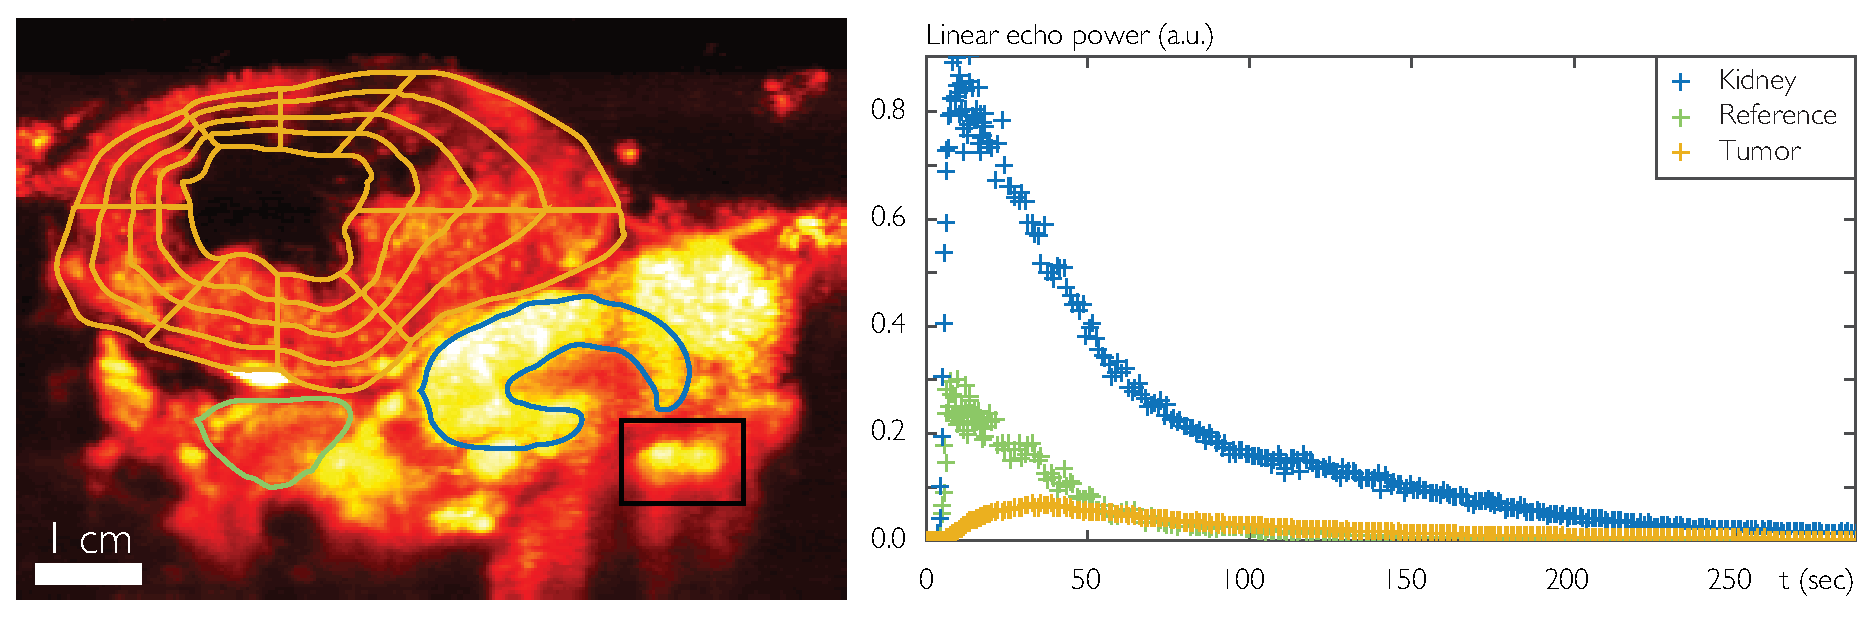
\includegraphics[width=\textwidth]{Figure1.eps}
	\caption{Illustration of the data pre-processing steps. Left: The contours of the tumor and its necrotic core have been overlaid on a  contrast enhanced image (in ochre color). The perfused tumor area was divided into 4 radial layers and 8 angular sectors. A reference tissue region (in green color) and a renal cortex region (in blue color) were also delineated. Right: Mean kinetics associated with the non-necrotic part of the tumor, the reference tissue, and the renal cortex.} 
  	\label{fig:Ch3Segmentation}
\end{figure}

\section{Methods}

\subsection{Quantification of tumor perfusion}
\label{sec:models}
Table \ref{tab:MODELS} summarizes the main features of the eight methods tested, three absolute and five relative, for tumor perfusion quantification. Some methods require the definition of an arterial region in order to estimate the AIF, its estimation is presented in section~\ref{sec:AIFmodel}. Relative quantification methods require the selection of a reference tissue region (labeled with subscript R). This region was segmented in order to define a homogeneous area, while being large enough in order to reduce noise influence on the subsequent analysis (Figure~\ref{fig:Ch3Segmentation}).

For all methods, quantitative parameters were derived by the minimization of the root-mean-square error between the time-intensity curve inside the tumor, $C_T(t)$, and the corresponding fitted curve, using an interior-point algorithm (MATLAB, MathWorks, Natick, MA, USA). To make the comparison between models easier, we focused on volume-based, flow-based, and time delays parameters.


\begin{table}
\begin{center}
\setlength{\tabcolsep}{3pt}
\begin{tabular}{llccll}
\toprule
 Acronym & Model Name & Input data & Eq. & Parameters \\
 & & AIF/RT & & & \\
\midrule
\bf{aLN} & Log-Normal & No/No &  (\ref{eq:Ch3LNmodel}) & $AUC,WIR, \Delta$ \\
\bf{aAIF} &  One-Compartment & Yes/No & (\ref{eq:CMM}) & $V,F$ \\
\bf{aAIFd} & One-Compartment with delay & Yes/No & (\ref{eq:CMM}) & $V, F, d$\\
\midrule
\bf{rLN} & Relative Log-Normal & No/Yes &  (\ref{eq:Ch3LNmodel},\ref{eq:LNr}) & $rAUC,rWIR, D$ \\
\bf{rAIF}& Relative One-Compartment & Yes/Yes & (\ref{eq:CMM},\ref{eq:AIFr})  & $ rV_{AIF},rF_{AIF}$ \\
\bf{rAIFd} &Relative One-Compartment with delay & Yes/Yes & (\ref{eq:CMM},\ref{eq:AIFr})  &  $ rV_{AIF},rF_{AIF},D_{AIF}$\\
\bf{rRT} & Relative Reference Tissue & No/Yes & (\ref{eq:RTDEF2},\ref{eq:RTparam})  & $ rV_{RT},rF_{RT}$ \\
\bf{rRTd} & Relative Reference Tissue with delay & No/Yes & (\ref{eq:RTDEF2},\ref{eq:RTparam}) & $ rV_{RT},rF_{RT},D_{RT}$ \\
\bottomrule
\end{tabular}
\caption{Synthesis of the different models tested. The first three models propose absolute quantification. The last five models propose relative quantification.}
\label{tab:MODELS}
\end{center}
\end{table}

\subsubsection{Absolute Log-normal model: aLN~\cite{Strouthos2010it}.}
The kinetics $C_T(t)$ is fitted according to the equation (\ref{eq:Ch3LNmodel}):
% \setlength{\mathindent}{30pt}
\begin{equation}
\begin{array}{rcl}
C_T(t) &= & \frac{AUC_T}{\sqrt{2 \pi}\sigma_T (t- \Delta_T)} \exp \left( - \frac{\left[ \ln{(t- \Delta_T)} - \mu_T \right]^2}{2{\sigma_T}^2} \right) \textrm{if } t > \Delta_T, \\
&=& \textrm{0 otherwise,}
\end{array}
\label{eq:Ch3LNmodel}
\end{equation}
where $AUC_T$ is the area under the $C_T$ curve, $\mu_T$  and $\sigma_T$ are the expectation and standard deviation of the distribution $C_T(\tau)/AUC_T$ when substituting $\ln(t- \Delta_T)$ with $\tau$, and $\Delta_T$ represents the time shift between the start of the acquisition and the arrival of the contrast agent in the tumor. As the area under the curve $AUC_T$ is related to the tissue blood volume~\cite{Tudorica2002at} and the wash-in rate $WIR_T$ (derived from $AUC_T$, $\mu_T$ and $\sigma_T$) is related to the tissue blood flow~\cite{Dietrich2012kw}, these two parameters were estimated in addition to $\Delta_T$ in the remaining analysis.

\subsubsection{One-Compartment model with an Arterial Input Function: \textbf{aAIF} and \textbf{aAIFd}}~\cite{Gunn2001gr}. The mathematical expression of $C_T(t)$ is given by equation (\ref{eq:CMM}):
\label{sec:AIFmodel} 
\begin{equation}
\label{eq:CMM}
\begin{array}{rcl}
C_T (t)  &= & F_T \int_{0}^{t- d_T} C_A \left( \tau \right) \exp^{-\frac{F_T}{V_T} \left( t - d_T - \tau \right)}\mathrm d \tau \quad \textrm{if } t \geq d_T,\\
&=& \textrm{0 otherwise,}
\end{array}
\end{equation}
where $C_A(t)$ is the kinetics inside the feeding artery (the AIF), $V_T$ the tissue blood volume (in \%), $F_T$ the tissue blood flow (in s$^{-1}$), and $d_T$ (in s) the time-delay of the contrast agent from the feeding artery to the tumor. When it is neglected ($d_T=0$), the model is noted \textbf{aAIF}. When it is estimated in addition to $V_T$ and $F_T$, the model is noted \textbf{aAIFd}.

To estimate the AIF, a bounding box surrounding arterial vessels was first defined according to anatomical considerations and high values of enhancement (see Figure~\ref{fig:Ch3Segmentation}).
Peak Enhancement ($PE$) and Time To Peak ($TTP$) parametric maps were then computed for each pixel of the bounding box.  The maximal value of $PE$ ($PE_{max}$) and the minimal value of $TTP$ ($TTP_{min}$) were extracted. Pixels verifying $PE/PE_{max}\geq rPE^{*}$ and $TTP-TTP_{min}\leq\Delta TTP^{*}$ were considered as part of the artery region (Figure~\ref{fig:AIF}), where $rPE^{*}$ and $\Delta TTP^{*}$ are empirically chosen cut-off values, equal to $50\%$ and 3 s, unless specified differently.
The AIF, $C_A(t)$, was computed as the geometric mean of the kinetics inside the artery region and modeled using the LN model  (\ref{eq:Ch3LNmodel}).  

\begin{figure}[ht]
  \centering
  \includegraphics[width=\linewidth]{Figure2.eps}
  \caption{Automated detection of the AIF: parametric maps $TTP$ and $PE$ inside the artery region; segmentation results and associated AIF with: (a) $rPE^{*}=50\%$ and $\Delta TTP^{*}=3$ s  (in green color); (b) $rPE^{*}=70\%$ and $\Delta TTP^{*}=2.5$ s  (in blue color).}
\label{fig:AIF}
\end{figure}

\subsubsection{Relative Log-Normal model: \textbf{rLN}.}  
This model estimates three relative parameters: the relative area under the curve $rAUC$, the relative wash-in rate $rWIR$, and the time delay between the arrival of the contrast in the tumor and the reference tissue $D_{T-R }$ according to equation~(\ref{eq:LNr}):

\begin{equation}
rAUC = \frac {AUC_T} {AUC_{R}}, \quad rWIR = \frac{WIR_T}{WIR_{R}}, \quad \textrm{and } \quad D^{T-R}_{LN} = \Delta_T - \Delta_{R},
\label{eq:LNr}
\end{equation}
where ($AUC_T$, $WIR_T$, $\Delta_T$) and  ($AUC_{R}$, $WIR_{R}$, $\Delta_{R}$) are the absolute LN parameters estimated in the tumor and in the reference tissue respectively using equation~(\ref{eq:Ch3LNmodel}).

\subsubsection{Relative One-Compartment model with an Arterial Input Function: \textbf{rAIF and rAIFd}.}
\label{sec:rAIFmodel}
This model estimates three parameters: the relative blood volume $rV_{AIF}$, the relative blood flow $rF_{AIF}$  and the  time delay between the arrival of the contrast in the tumor and the reference tissue $D^{T-R}_{AIF}$ according to equation~(\ref{eq:AIFr}):
\begin{equation}
rV_{AIF} = \frac {V_T} {V_{R}}, \quad rF_{AIF} = \frac {F_T} {F_{R}}, \quad \textrm{and } \quad D^{T-R}_{AIF} = d_T - d_{R},\\
\label{eq:AIFr}
\end{equation}
where ($V_T$, $F_T$, $d_T$) and ($V_{R}$, $F_{R}$,  $d_{R}$)  are the perfusion parameters estimated in the tumor and in the reference tissue respectively using the AIF according to equation~(\ref{eq:CMM}).
This method is referred to as \textbf{rAIF} when $D^{T-R}_{AIF} $ is set to zero and \textbf{rAIFd} otherwise. 

\subsubsection{Relative One-Compartment model using the Reference Tissue kinetics: \textbf{rRT and rRTd}}~\cite{Patlak1983id,Yankeelov2005de}.
This model estimates three parameters: the relative blood volume $rV_{RT}$, the relative blood flow $rF_{RT}$ and the time delay between the arrival of the contrast in the tumor and the reference tissue $D^{T-R}_{RT}$, the subscript $_{RT}$ being used for distinguishing this approach from the previous one (section~\ref{sec:rAIFmodel}). Assuming that the tumor and the reference region have a common AIF, the kinetics $C_{R}(t)$ and $C_{T}(t)$ can be described by equation~(\ref{eq:CMM}). When replacing $C_A(t)$ by its expression as a function of $C_R(t)$ in equation~(\ref{eq:CMM}), $C_T(t)$  can then be described by equation (5):
\begin{equation}
\begin{array}{rcl}
\hspace{-10mm}
C_T \left( t \right) & = & rF_{RT} \Big[ C_{R} \left( t - D_{RT}^{T-R} \right) \\
& & \qquad + \left( k_{R} - k_T \right) \int_{d_{R}}^{t - D_{RT}^{T-R}} C_{R} \left( \tau \right) e^{- k_T \left( t - D_{RT}^{T-R} - \tau \right)} \mathrm d \tau \Big] \quad \textrm{ if } t \geq d_T, \\
& = & \textrm{0 otherwise,}
\end{array}
\label{eq:RTDEF2}
\end{equation}
where $k_{R} = F_{R}/V_{R}$ and $k_T = F_T/V_T$. The parameter $k_{R}$ was chosen as the mean value of the $k_{R}$ values estimated with the relative AIF approach (\textbf{rAIFd}) and was set to 0.15. The parameters $rF_{RT}$, $k_T$ and$D^{T-R}_{RT}$ were estimated by solving equation~(\ref{eq:RTDEF2}). The parameter $rV_{RT}$ was then deduced using equation~(\ref{eq:RTparam}): 
\begin{equation}
rV_{RT} = \frac{V_T}{V_{R}}  = \frac{F_{T}}{k_{T}} \frac{k_{R}}{F_{R}} = rF_{RT}\frac{k_{R}}{k_T}.
\label{eq:RTparam}
\end{equation}
The method is referred to as \textbf{rRT} when $D^{T-R}_{RT}$ is set to zero and \textbf{rRTd} otherwise. 

\subsection{Data analysis}
For each model, the quantitative assessment of the fit was achieved using the normalized root mean square error ($NRMSE$), and the fraction of information that is modeled  ($FMI$), as defined in~\cite{Balvay2005ca}. The $NRMSE$ was defined by: 
\begin{equation}
NRMSE = \frac{\sqrt{\frac{1}{nt} \sum_{t=1}^{nt}\left(C_{fit}\left(t\right)-C\left(t\right)\right)^2}}{max_t(C(t))-min_t(C(t))},
\end{equation}
where $C$ and $C_{fit}$ are the observed and fitted kinetics and $nt$ is the total number of frames. 
A good fit corresponds to $NRMSE$ close to 0 and $FMI$ close to 100\%.
For each sub-region, results for which $FMI < 90\%$ were judged as poor quality fits.


In order to assess the reproducibility of the parameters $\theta^{hl}$ of the mouse $m_l$ ($l$ from 1 to 4) in the sub-region $s_h$ ($h$ from 1 to 32), coefficients of variation $CV^{hl}$  were estimated using the four test-retest studies, as follows: 
\begin{equation}
{CV^{hl}} = \frac {\sqrt {\frac{1}{4} {\sum _{k=1}^{4} (\theta^{hl}(k)- \mu^{hl})^2}}} {\mu^{hl}}, \textrm {where } \mu^{hl}=\frac{1}{4} \sum _{k=1}^{4} \theta^{hl}(k),
\label{eq:Ch3CV}
\end{equation}
$\theta^{hl}(k)$ being the parameter $\theta^{hl}$ estimated for the $kth$ test-retest study (with $k$ from 1 to 4).
As parameters $\theta^{hl}(k)$ corresponding to poor quality fits were removed, missing values were replaced using multivariate imputation according to the R package \{mice\}, 'Multivariate Imputation by Chained Equations'~\cite{vanBuuren2011ica}, in order to compute $CV^{hl}$ using four values systematically.

Statistical tests were performed to compare goodness of fit criteria and coefficients of variation between the different models, using the R package \{coin\}, 'Conditional Inference Procedures in a Permutation Test Framework'~\cite{Hothorn2008ht}. They were considered as significant when p values were less than $0.05$. As all the tests were conducted on paired data, when goodness of fit criteria were removed (due to poor quality fits), they were replaced with imputed data.
The non-parametric Friedman test with post-hoc analysis (Tukey's HSD test) was chosen for dealing with multiple comparisons. 

\section{Results}
\label{sec:results}
\subsection{Model comparison through quality of fit criteria}
\begin{table}
\begin{center}
\setlength{\tabcolsep}{4pt}
\begin{tabular}{l | rr | rrrrr}
\toprule
\multirow{2}{*}{Model} & \multicolumn{2}{c |}{All data} &  \multicolumn{3}{c}{$FMI > 90\%$}\\
& \multicolumn{2}{c |}{$NRMSE$  \quad \quad \quad \quad $FMI$} &  \multicolumn{2}{c}{$NRMSE$   \quad \quad \quad \quad $FMI$}  & $N$ \\
\midrule
\textbf{aLN}    & 5.75  [4.70-7.41]  &	99.4 [98.5-99.8] & 5.63  [4.62-7.00]	& 99.4 [98.8-99.8] &	28\\	
\textbf{aAIF} & 9.95$^{\star \dagger}$ [6.03-24.2] &  94.7$^{\star \dagger}$  [45.2-98.3] &  6.72$^\circ$ [5.12-9.20] &  97.8$^\circ$ [95.5-98.9] & 212 \\
\textbf{aAIFd} & 6.21	[4.71-8.43] & $98.7^\star$ [97.3-99.4] &  6.04  [4.66-8.20] &  $98.8^\star$ [97.6-99.4] & 19		\\
\textbf{rRT} & 7.72$^{\star \ddagger}$  [5.83-9.85] & 97.6$^{\star \ddagger}$  [94.9-98.7] &  7.45$^{\star \ddagger}$ [5.71-9.34] & 97.8$^{\star \ddagger}$ [95.6-98.8] & 56 \\
\textbf{rRTd} & 6.32 [4.91-8.21] & 98.7$^\star$ [97.2-99.4] &  6.18 [4.85-8.00]	& $98.8^\star$ [97.6-99.4]	& 19 \\
\bottomrule
\end{tabular}
\caption{Median [first-third quartiles] values of  $NMRSE$ and $FMI$ (in \%) obtained for the different models. $N$ is the  number of sub-regions where $FMI < 90\%$. Significant differences between \textbf{aLN} and any other model are indicated by $^\star$. In addition, significant differences between \textbf{aAIF} (resp. \textbf{rRT}) and \textbf{aAIFd} (resp. \textbf{rRTd)} are indicated by $^\dagger$ (resp. $^\ddagger$). The symbol $^\circ$ indicates that comparisons were not reported due to the high number of missing data.}
\label{tab:FIT}
\end{center}
\end{table}

Table~\ref{tab:FIT} shows the quartile values of the quality of fit criteria ($NRMSE$ and $FMI$), which are computed for the 512 ($4\times 4\times 32$) tumor sub-regions for the five models: \textbf{aLN}, \textbf{aAIF}, \textbf{aAIFd}, \textbf{rRT}, and \textbf{rRTd}.
Since the $NMRSE$ and $FMI$ criteria obtained by the three relative methods \textbf{rLN}, \textbf{rAIF} and \textbf{rAIFd} are identical to those obtained by \textbf{aLN}, \textbf{aAIF} and \textbf{aAIFd}, these results are not reported in Table~\ref{tab:FIT}. Additionally, quartile values are provided for the $N$ sub-regions verifying $FMI > 90\%$. 
Due to the large portion of missing data for the \textbf{aAIF} model when considering only good fits (the number of excluded regions, $N$, being equal to 212), results of hypothesis testing were not presented for that specific case. 
The \textbf{aLN} model shows slightly better quality criteria than the other models (these differences are significant for $FMI$ in all cases, and significant for $NRMSE$ in case of \textbf{aAIF} and \textbf{rRT} models). The introduction of the time delay parameter (\textbf{aAIFd},  \textbf{rAIFd} and \textbf{rRTd} models) significantly improved the modeling quality, according to both criteria. Furthermore, the number of cases for which $FMI <90\%$ was largely reduced when taking into account the time delays. For these reasons, results obtained without time delays (\textbf{aAIF}, \textbf{rAIF} and \textbf{rRT}) were not further reported.

\subsection{Model comparison through coefficients of variation}

All mean values and standard deviations of the perfusion parameters are given for each mouse in Appendix, in Table~\ref{tab:RP}.  
Figure \ref{fig:Slopes} illustrates for one specific mouse ($m_1$) the comparison between the parameters estimated by the different models. It shows a high correlation between the  volume-based parameters: $AUC$, $rAUC$, $V$, $rV_{AIF}$, and $rV_{RT}$ as well as a high correlation between the  flow-based parameters: $WIR$, $rWIR$, $F$, $rF_{AIF}$, and $rF_{RT}$. This figure shows also that there is a large range of values for each parameter within one tumor, demonstrating that perfusion parameters inside the different sub-regions of the tumor are far from being similar. Finally, it proves  that the slopes may be quite different from one study to another, and that the use of relative parameters contributes to largely reduce the differences between the test-retest studies, the estimation of $rF_{AIF}$ being less robust than the estimation of $rWIR$ or $rF_{RT}$ for this specific example. Table~\ref{tab:AIF} illustrates the influence of the AIF choice on the estimation of volume, flow, and time delay parameters. On this specific exam, two AIF were generated, the first one (AIF$_1$) with thresholds $rPE^{*}=50\%$ and $\Delta TTP^{*}=3$ s, the second one (AIF$_2$) with thresholds $rPE^{*}=70\%$ and $\Delta TTP^{*}=2.5$ s (as shown in Figure~\ref{fig:AIF}). The variations were very large for $V$ and $F$ parameters, while they remained moderate for $rF_{AIF}$ and time delays, and very low for $rV_{AIF}$.

\begin{figure}[ht]
  \centering
  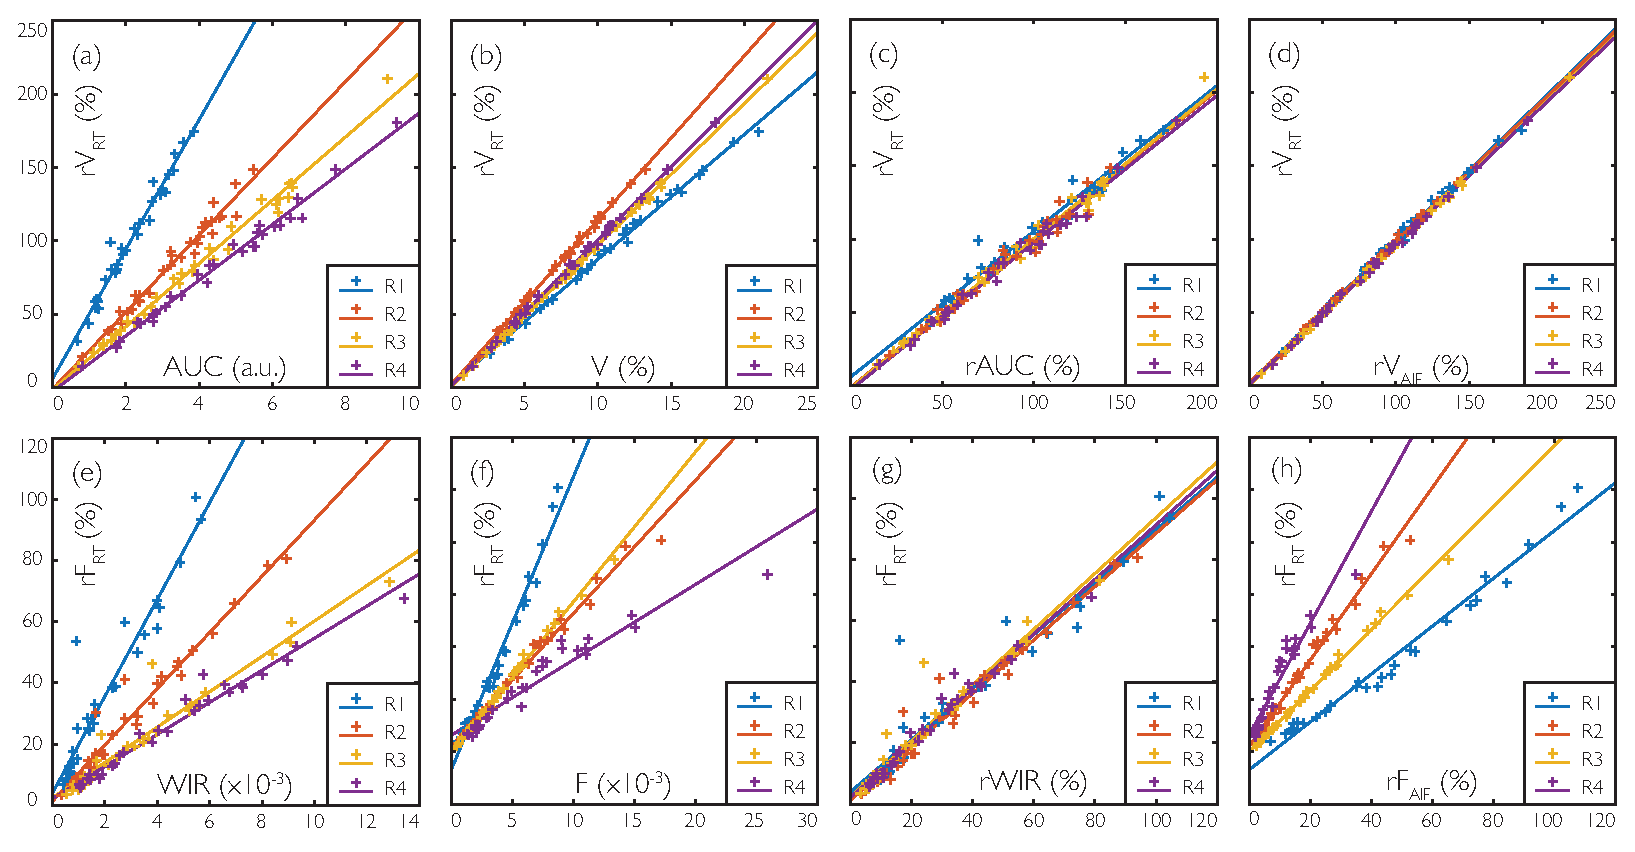
\includegraphics[width=\linewidth]{Figure3.eps}
  \caption{Comparison of the volume-based and flow-based parameters obtained for the four test-retest exams ($R_1$, $R_2$, $R_3$, and $R_4$) of the mouse $m_1$: linear regressions between (a) $rV_{RT}$ and $AUC$, (b) $rV_{RT}$ and $V$, (c) $rV_{RT}$ and $rAUC$, (d) $rV_{RT}$ and $rV_{AIF}$, (e) $rF_{RT}$ and $WIR$, (f) $rF_{RT}$ and $F$, (g) $rF_{RT}$ and $rWIR$, (h) $rF_{RT}$ and $rF_{AIF}$.}
\label{fig:Slopes}
\end{figure}

\begin{table}[ht]
\begin{center}
\begin{tabular}{ccccccc}
\toprule
& $V$ (\%) & $rV_{AIF} (\%) $ & $F$ ($10^{-3}$ s$^{-1}$) & $rF_{AIF}$ (\%)& $d_T$ (s) & $D_{AIF}^{T-R}$ (s) \\
\midrule
AIF$_1$ & $8.02 \pm 3.89$ 	& $84.5 \pm 40.9$ 
		& $6.54 \pm 5.37$ 	& $8.83 \pm 7.24$ 
		& $2.4 \pm 3.4$ 	& $1.4 \pm 3.4$ \\
AIF$_2$ &$4.65 \pm 2.25$ 	& $85.2 \pm 41.3$ 
		& $3.20 \pm 2.61$ 	& $10.1 \pm 8.21$ 
		& $2.0 \pm 3.3$ 	& $1.6 \pm 3.3$ \\
\bottomrule
\end{tabular}
\caption{Mean $\pm$ standard deviation of the parameters estimated with the \textbf{aAIFd} and  \textbf{rAIFd} models, using two different sets of cut-offs to generate the AIF functions.}
\label{tab:AIF}
\end{center}
\end{table}

\begin{figure}[ht]
  \centering
  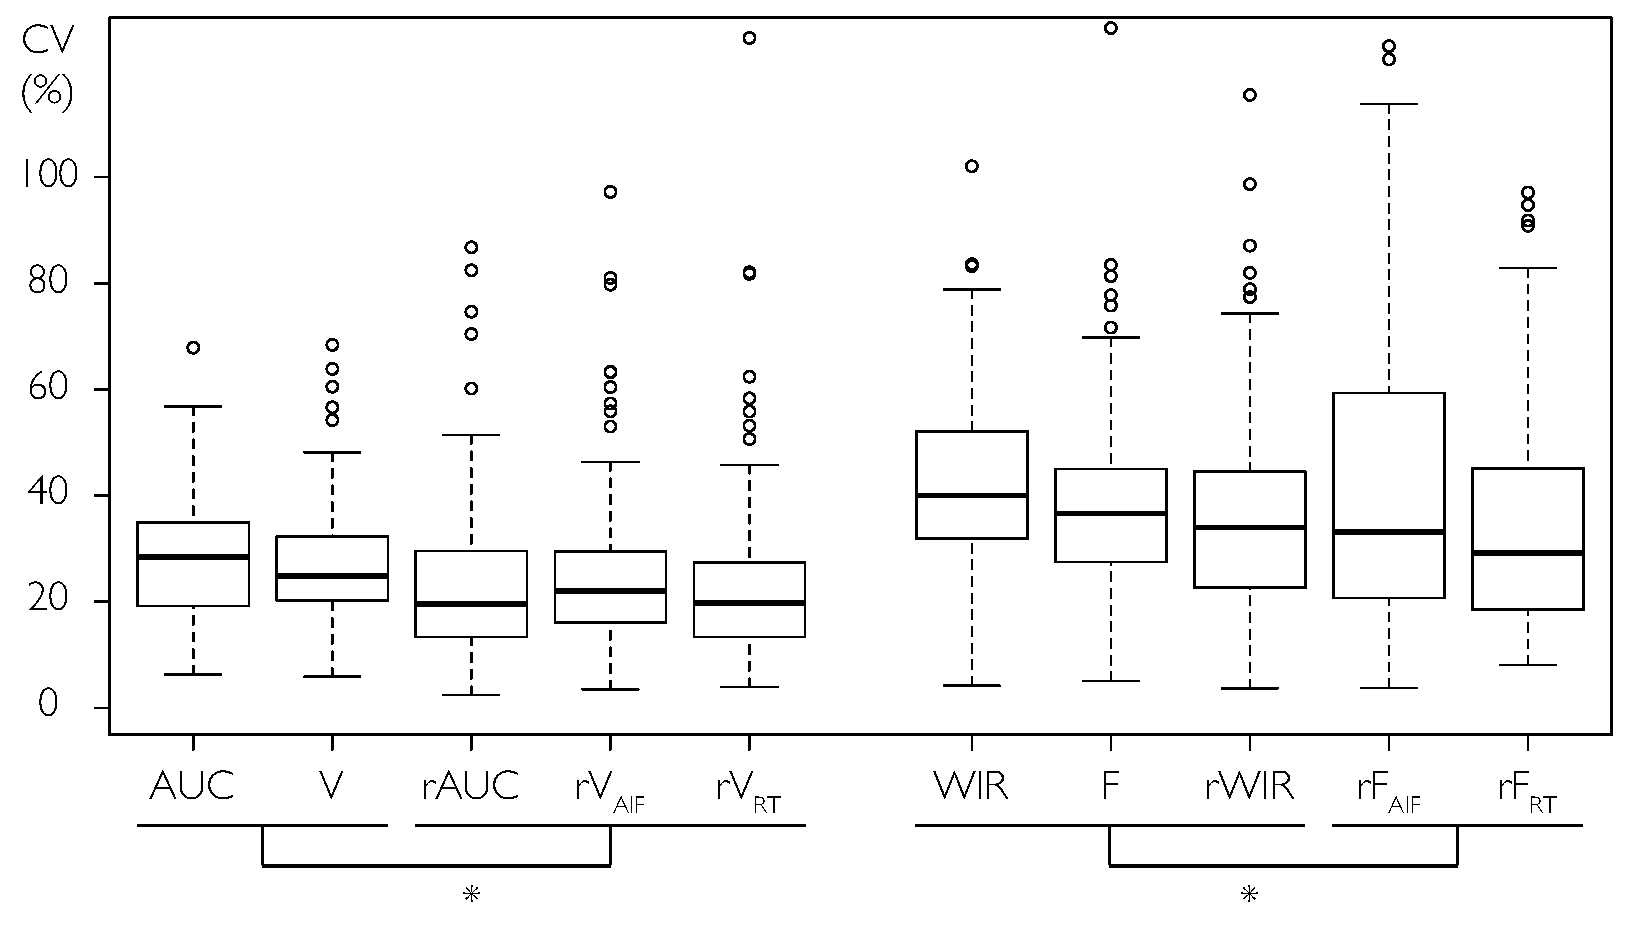
\includegraphics[width=\linewidth]{Figure4.eps}
  \caption{Boxplot showing the coefficients of variation of blood volume parameters (left) and blood flow parameters (right) estimated with the \textbf{aLN}, \textbf{rLN}, \textbf{aAIFd}, \textbf{rAIFd}, and \textbf{rRTd} models. For each box, the bold line represents the median value, the bottom and top lines the first and third quartiles. Dotted lines extend to the most extreme data points which are less than 1.5 times the interquartile range. Outlier points are displayed with empty circles. Two groups of parameters were built (horizontal lines below the parameter names) such that there were no significant intra-group differences while there were statistically significant inter-group differences (marked by $^{*}$).}
\label{fig:CV}
\end{figure}

Finally, Figure~\ref{fig:CV} shows the distributions of the coefficients of variation of volume-based and flow-based parameters, computed according to equation (\ref{eq:Ch3CV}). Relative volume parameters ($rAUC$, $rV_{AIF}$, and $rV_{RT}$) have significantly lower CV than absolute volume parameters ($AUC$ and $V$). No significant difference was found when comparing $WIR$, $F$, and $rWIR$, but the CV of these parameters are significantly higher than those of $rF_{AIF}$ and $rF_{RT}$.
Numerical values of these mean CV are given for each mouse in Appendix, in Table~\ref{tab:RCV}.


\section{Discussion}
Using a test-retest study with a controlled bolus injection, it was possible to assess the variability of DCE-US perfusion parameters. To reduce this variability, the interest of estimating relative parameters, which necessitates the definition of a reference tissue region, was practically demonstrated. Our study also shows the importance of choosing an appropriate method for the estimation of the parameters, because estimation methods have an impact on parameter variability. Thus the reference tissue approach (\textbf{rRTd}) can be recommended, since it is the most robust method when considering the volume-based and the flow-based parameters simultaneously.

The recommendations of the EFSUMB for DCE-US quantification in oncology suggest to estimate  parameters such as $AUC$ and $WIR$ from explicitly defined models, e.g.~using the \textbf{aLN} model. To reduce the variability of the estimated parameters, Dizeux et al. proposed a controlled injection system~\cite{Dizeux2016cd}. However, the present study shows that the differences between two consecutive exams are still not negligible for a regional analysis. Since in PET and DCE-MRI, deconvolution approaches and compartmental models have proved their efficiency to make parameters more robust to inter-exam changes, we decided to test some of these approaches. The most commonly used methods require the estimation of an arterial input function. Deconvolution approaches were recently proposed to quantify tissue perfusion in DCE-US~\cite{Gauthier2012vc}. These approaches estimate the transfer function of the system (depending on a large number of parameters), and to avoid aberrant solutions, this estimation needs to be regularized. 
Following this idea, the one-compartment model with time delay is a deconvolution depending on three parameters only. When the time delay is set to 0,  (\textbf{aAIF} model), we have shown that the quality of fit is worse than the one obtained when using the explicit \textbf{aLN} model. 
When introducing a time delay parameter, an option that is unfortunately generally overlooked~\cite{Kudo2009hy}, a much more accurate fit of regional tumor kinetics was obtained. Indeed, the quality of fit using \textbf{aLN} (depending on four parameters) and this  \textbf{aAIFd} model was equivalent in terms of $NRMSE$. 

Our study shows the crucial role of the AIF estimation in the variability of the perfusion parameters (see Table~\ref{tab:AIF}). When focusing the field of view in the main plane of the tumor, it can be difficult to estimate the AIF robustly (see Figure~\ref{fig:AIF}). Indeed, AIF measurements in small vessels can be affected by partial volume effects, yielding underestimation of the signal intensity. Thus coefficients of variation deduced from the \textbf{aAIFd} model can be high. Note that some problems could also occur in larger vessels, including non-linearities between concentration and measured signal, and attenuation artifacts ~\cite{Mule2008ms}.

The use of relative parameters was suggested to overcome the difficulties of estimating the AIF for a compartmental model in DCE-MRI ~\cite{Yankeelov2005de}. Clinical studies have reported the interest of estimating normalized perfusion parameters in DCE-US \cite{Guibal2010bl,Hoeffel2010ce,Lefort2012km}. Using systematically three models (\textbf{rLN}, \textbf{rAIFd}, \textbf{rRTd}), our study reinforces the interest of estimating relative parameters. The choice of a reference tissue region is less critical than the segmentation of an artery. Indeed, a larger structure can be used, reducing segmentation errors and the impact of partial volume effect. Furthermore, as the contrast concentration is lower, the quantification errors due to non-linearity are reduced. Kidney regions were initially tested but finally excluded because of the overlap of cortical, proximal tubular and distal tubular compartments. Muscular regions that could be delineated on the four exams were finally chosen.

Recirculation is a major problem when dealing with modeling techniques adapted to first-pass studies. However, its quantitative impact is reduced in DCE-US when compared to other modalities since the destruction of microbubbles, in the lungs in particular, makes the number of microbubbles much smaller in the second pass (and following) than it is in the first pass. We deliberately did not try to model the recirculation, when we chose the \textbf{aLN} model to fit tumor kinetics or when we first fit the AIF using the \textbf{aLN} model. In addition, using simulated data, we showed that the practical impact on parameters estimation when neglecting the recirculation was limited, especially for relative parameters, since the coefficients of variation between parameters estimated with and without simulating the recirculation effect were less than the ones estimated through the test-retest studies (this recirculation effect was about 5\% on CV values with the \textbf{rRTd} approach).

The use of normalized parameters induced a significant reduction of coefficients of variation in our test-retest study. 
Furthermore, estimating relative volume and flow parameters using equation~(\ref{eq:RTDEF2}), which eliminates the need for an AIF, is more robust than using the AIF directly. It should also be noted that the small 3D displacements occurring between the four test-retest studies can partly explain the CV, due to the imperfect spatial alignment between sub-regions from one exam to the following one.

 Figure~\ref{fig:Slopes} reveals strong correlations between the different parameters computed inside a same sub-region, and a large variation of these parameters according to the tumor sub-regions. Thus, whatever the model used,  all the flow-based or volume-based parameters can reveal spatial tumor heterogeneity. However, when it comes to the comparison of longitudinal exams, it is crucial to have comparable parameter values. Thus, the estimation of relative parameters seem to be the most powerful solution, provided that the reference tissue characteristics are not modified between exams.
Some interesting results have been recently shown~\cite{Wang2015bb} for a longitudinal study using a 3D DCE-US approach. Compared with the 2D approach, the 3D approach enables assessment of the whole tumor and should be preferred for tumor monitoring.

 \section{Conclusion}
This study aimed at proposing valuable modeling of DCE-US studies to estimate reliable perfusion parameters in a murine model of tumor. First, it was shown that a one-compartment model based on an AIF, and completed by the estimation of a time-delay parameter, could fit kinetics as closely as the explicit log-normal model. Second, a comprehensive comparison of the parameters estimated by different approaches was proposed, showing high correlations between the volume-based  and flow-based parameters respectively estimated. Based on test-retest studies with controlled injections, a large variability (up to 40\%) of regional perfusion parameters was established due to the inherent variations of experimental and physiological conditions for the log-normal modeling and to the difficulties in estimating a correct AIF in the image field of view for the compartmental approach. To reduce this variability, the use of relative values of these regional perfusion parameters was proposed, requiring in all cases the delineation of a reference tissue region. To estimate these relative parameters, the reference tissue model proved to be the most reliable computing approach. Thus we recommend the use of this model to estimate reliable relative perfusion parameters.

\section{Acknowledgments}
The authors are grateful to the anonymous reviewers for their valuable comments on the paper.
This work was funded by the Fondation pour la Recherche M\'edicale through the Bioing\'enierie pour la Sant\'e research grant DBS20131128436. Research was also supported by the Institut Universitaire d{'}Ing\'enierie en Sant\'e, Sorbonne Universit\'e, Projet OCSCC 2014/2016.
Experiments were performed on a platform of France Life Imaging partly funded by the grant ANR-11-INBS-0006 associated within the Plateforme Imagerie du Vivant. All the animals were house kept at Centre d{'}Ex-plorations Fonctionnelles of Centre de Recherche des Cordeliers, Agreement A75-06-12.

\section* {Appendix}
This appendix gives the numerical results that were obtained for each mouse ($m_1$, $m_2$, $m_3$, and $m_4$), including mean values and standard deviations of regional parameters (Table \ref{tab:RP}) and coefficients of variation of these parameters (Table \ref{tab:RCV}). 

\begin{table} [hb]
\begin{center}
\begin{tabular}{lccccc}
\toprule
& \multicolumn{2}{c}{Absolute parameters} & \multicolumn{3}{c}{Relative parameters} \\
\midrule
 & $AUC$ (a.u.) & $V$ (\%)  & $rAUC$ (\%) & $rV_{AIF}$ (\%)  & $rV_{RT}$ (\%)  \\
\midrule
$m_1$  	& $3.47 \pm 1.82$ 	& $8.61 \pm 4.31$ 	& $87.2 \pm 37.9$ 	& $87.6 \pm 41.5$ 	& $85.9 \pm 41.2$ 	\\
$m_2$  	& $5.97 \pm 2.08$ 	& $17.6 \pm 6.60$ 	& $11.2 \pm 3.19$ 	& $18.1 \pm 6.25$ 	& $13.2 \pm 3.51$ 	\\
$m_3$  	& $6.74 \pm 3.51$ 	& $12.9 \pm 6.40$ 	& $144 \pm 81.3$ 	& $131 \pm 73.0$ 	& $132 \pm 75.2$ 	\\
$m_4$  	& $7.90 \pm 4.23$ 	& $21.2 \pm 11.6$ 	& $57.9 \pm 30.6$ 	& $62.3 \pm 33.1$ 	& $59.4 \pm 31.6$ 	\\
\midrule
& $WIR$ (a.u. s$^{-1}$)  & $F$ (s$^{-1}$) & $rWIR$ (\%) & $rF_{AIF} (\%) $ & $rF_{RT}$ (\%) \\
\midrule
$m_1$ 	& $3.30 \pm 2.66$ 	& $4.94 \pm 4.07$ 	& $29.7 \pm 23.4$ 	& $21.9 \pm 21.9$ 	& $27.0 \pm 20.3$ 	\\
$m_2$ 	& $4.70 \pm 3.03$ 	& $6.49 \pm 3.45$ 	& $17.7 \pm 10.2$ 	& $17.2 \pm 8.34$ 	& $16.1 \pm 11.0$ 	\\
$m_3$  	& $4.88 \pm 4.19$ 	& $3.64 \pm 2.90$ 	& $32.9 \pm 28.6$ 	& $36.4 \pm 27.7$ 	& $25.1 \pm 21.0$ 	\\
$m_4$  	& $6.63 \pm 5.30$ 	& $5.21 \pm 3.59$ 	& $23.7 \pm 19.0$ 	& $26.4 \pm 18.2$ 	& $18.0 \pm 13.6$ 	\\
\midrule
Delay & $\Delta$ (s) & $d$ (s)& $D^{T-R}_{LN}$ (s)& $D_{AIF}^{T-R}$ (s)  & $D_{RT}^{T-R}$ (s) \\
\midrule
$m_1$  	& $5.5 \pm 3.4$		& $3.2 \pm 4.1$		& $-1.9 \pm 3.4$	& $2.7 \pm 4.2$ 	& $3.9 \pm 4.7$	\\
$m_2$  	& $2.8 \pm 2.5$		& $5.7 \pm 4.7$		& $0.7 \pm 2.4$		& $4.2 \pm 4.5$ 	& $5.3 \pm 4.0$ \\
$m_3$ 	& $3.2 \pm 2.8$		& $7.4 \pm 5.6$		& $0.4 \pm 3.1$		& $3.6 \pm 5.5$ 	& $4.4 \pm 5.8$ \\
$m_4$  	& $4.4 \pm 2.4$		& $7.0 \pm 4.6$		& $-0.8 \pm 2.3$	& $5.9 \pm 4.5$ 	& $5.6 \pm 4.7$ \\
\bottomrule
\end{tabular}
\caption{Mean $\pm$ standard deviation of the volume, flow and delay parameters estimated in the different sub-regions of the tumor, for the four test-retest exams, after multiple imputation of missing values due to poor fit quality. Values of $WIR$ and $F$ are multiplied by 1000.}
\label{tab:RP}
\end{center}
\end{table}

\begin{table}
\begin{center}
\begin{tabular}{lccccc}
\toprule
& \multicolumn{2}{c}{Absolute parameters} & \multicolumn{3}{c}{Relative parameters} \\
\midrule
 & $CV_{AUC}$  & $CV_{V}$  & $CV_{rAUC}$  & $CV_{rV_{AIF}}$  & $CV_{rV_{RT}}$ \\
\midrule
$m_1$  	& $34.7 \pm 10.6$ 	& $30.2 \pm 17.1$ 	& $22.4 \pm 14.4$ 	& $24.6 \pm 17.5$ 	& $24.7 \pm 17.3$ 	\\
$m_2$  	& $26.2 \pm 6.83$ 	& $26.7 \pm 9.85$ 	& $15.0 \pm 6.51$ 	& $21.8 \pm 9.99$ 	& $15.3 \pm 7.01$ 	\\
$m_3$ 	& $31.0 \pm 12.3$ 	& $26.6 \pm 10.9$ 	& $37.2 \pm 16.8$ 	& $35.2 \pm 17.8$ 	& $35.2 \pm 18.7$ 	\\
$m_4$ 	& $20.7 \pm 10.6$ 	& $23.3 \pm 9.93$ 	& $18.8 \pm 8.68$ 	& $19.0 \pm 7.61$ 	& $17.8 \pm 8.17$ 	\\

\midrule
 & $CV_{WIR}$  & $CV_{F}$  & $CV_{rWIR}$ & $CV_{rF_{AIF}}$ & $CV_{rF_{RT}}$ \\
\midrule
$m_1$ 	& $42.4 \pm 12.4$ 	& $35.4 \pm 12.5$ 	& $33.4 \pm 14.9$ 	& $75.5 \pm 19.9$ 	& $29.6 \pm 13.2$ 	\\
$m_2$ 	& $44.4 \pm 11.0$ 	& $34.4 \pm 7.23$ 	& $27.4 \pm 10.9$ 	& $23.4 \pm 9.94$ 	& $33.1 \pm 18.7$	\\
$m_3$ 	& $45.3 \pm 18.5$ 	& $46.9 \pm 17.7$ 	& $50.9 \pm 17.7$ 	& $36.8 \pm 16.6$ 	& $38.3 \pm 21.3$ 	\\
$m_4$  	& $34.9 \pm 18.9$ 	& $33.3 \pm 17.3$ 	& $38.3 \pm 21.2$ 	& $27.1 \pm 13.7$ 	& $29.4 \pm 15.8$ 	\\

\bottomrule
\end{tabular}
\caption{Mean $\pm$ standard deviation of the coefficients of variation (CV), expressed in percentage, of volume and flow parameters estimated for each sub-region after multiple imputation of missing values due to poor fit quality. CV were not computed for time delays, since their values can be either positive or negative.}
\label{tab:RCV}
\end{center}
\end{table}

